%==================== PARTE B: RUÍDO NO SO, PROGRAMA DO PLC E CORREÇÃO ====================
\section{O programa do PLC (\texttt{Prova2.st}): o que ele realmente faz}\label{secst}
O programa é um PI\_D paralelo construído com blocos da biblioteca IEC 61131-3 e executado por uma tarefa de \textbf{20 ms} (\texttt{TASK task0(INTERVAL := T\#20ms)}). A listagem completa está no Apêndice~\ref{apcodigos}. Resumo, bloco a bloco:
\begin{center}\small
\begin{longtable}{p{3.4cm}p{11.2cm}}
\toprule \textbf{Elemento} & \textbf{O que faz (e por quê importa)}\\\midrule\endhead
Escalas & \texttt{VP}, \texttt{SP} e \texttt{SO} são \texttt{UINT} (0--65535). Multiplicar por $0{,}001525$ dá \%. O ADC de 10 bits do Arduino entra como múltiplos de 64, logo \textbf{1 LSB $=64\cdot0{,}001525=0{,}0976\,\%$}.\\
\texttt{MF} (\texttt{\%QX0.0}) & Modo: \texttt{MF=1} = automático (malha fechada); \texttt{MF=0} = manual. Em manual o erro é forçado a 0.\\
Erro & $e=(SP-VP)\cdot M\_ACAO$ ($M\_ACAO=1$). Zona morta: se $|e|<0{,}09$, $e=0$. Como o menor erro não nulo é 1 LSB $=0{,}0976>0{,}09$, \textbf{a zona morta nunca atua}.\\
Proporcional & $K_p\,e$, com \texttt{kp = 3.523}.\\
Integral & Bloco \texttt{INTEGRAL}, \texttt{XIN = ki$\cdot e$} (zero se \texttt{STOP\_INTGR}), \texttt{CYCLE = 500 ms}, reinicia em 0 quando \texttt{MF=0}; a saída é multiplicada por $0{,}04$. Como o bloco é executado a cada 20 ms mas ``acredita'' em 500 ms, o ganho $0{,}04=0{,}02/0{,}5$ corrige a escala: o resultado é $\int K_i\,e\,dt$ com \texttt{ki = 0.03872}.\\
Derivada & \texttt{XIN} $=-k_d\cdot VP$ (zero em manual), bloco \texttt{DERIVATIVE} com \texttt{CYCLE = 500 ms}, saída multiplicada por $25$ ($=0{,}5/0{,}02$, mesma correção de escala), \texttt{kd = 39.16}. \textbf{Não existe filtro $\mu T_d$} no programa. O bloco \texttt{DERIVATIVE} da biblioteca padrão usa a diferença de 4 pontos
\[\tfrac{3\,(x_k-x_{k-3})+x_{k-1}-x_{k-2}}{10\,T_s},\ T_s=20\ \mathrm{ms}.\]\\
Bias (bumpless da saída) & \texttt{SO\_AUX := SO} em manual, mantendo o último valor em automático. O SC é $SO_{manual}+K_pe+I+D$. Logo, ao fechar a malha com $e=0$, o SC continua igual ao SO manual (transferência sem salto), e a integral parte de zero.\\
VP-tracking & \texttt{SP := SEL(MF, VP, SP)}: em manual o SP é sobrescrito pela VP. É o mecanismo do item 1.2.\\
Anti-windup & \texttt{STOP\_INTGR := (u $\ge100$) OR (u $\le10$)}; quando verdadeiro, \texttt{XIN} da integral vale 0: \textbf{a integral congela enquanto o SC está saturado} (não é o \emph{clamping} condicionado ao sinal do erro). É o mecanismo do item 1.3.\\
Saturação & \texttt{LIMIT(10.0, u, 100.0)}: SC entre 10 e 100\,\% (\texttt{SC = u$\cdot655{,}35$}).\\
2GL & \texttt{FF2GL} acumula $K_p(1-\mathtt{alfa})\,\Delta SP$ a cada mudança de SP em automático e é \emph{subtraído} de $u$. \texttt{alfa = 1} $\Rightarrow$ PI\_D comum (Seção~\ref{alfaplc}).\\\bottomrule
\end{longtable}\end{center}
\subsection{A derivada de 4 pontos sem filtro: resposta a 1 LSB}\label{deriv4}
Seja um degrau de $\Delta V=1$ LSB $=0{,}0976\,\%$ na VP lida, ocorrendo no scan $k_0$ (a entrada do bloco é $-k_dVP$). Aplicando a fórmula de 4 pontos, a saída vale
\[
D_{k_0}=-\frac{3\,k_d\Delta V}{10T_s},\quad D_{k_0+1}=-\frac{4\,k_d\Delta V}{10T_s},\quad D_{k_0+2}=-\frac{3\,k_d\Delta V}{10T_s},\quad D_{k_0+3}=0,
\]
isto é, um pulso de 3 scans (60 ms) com área $k_d\Delta V$. Com os números do programa,
\[
u_0\equiv\frac{k_d\,\Delta V}{10\,T_s}=\frac{39{,}16\cdot0{,}0976}{10\cdot0{,}02}=19{,}1\ \text{pontos},\qquad\text{pulsos: }57{,}3;\ 76{,}4;\ 57{,}3\ \text{pontos de SC}.
\]
(Se existisse o filtro $\mu=0{,}1$ do projeto, o pico seria $k_d\Delta V/(\mu T_d)=3{,}4$ pontos.) Qualquer combinação de degraus de $\pm1$ LSB em scans vizinhos produz saídas que são múltiplos inteiros de $u_0=19{,}1$ pontos (coeficientes $3,1,-1,-3$ vezes $u_0$).

\subsection{O 2GL do programa e a tradução do $\alpha$ do TCC}\label{alfaplc}
Em automático, a cada mudança de SP o programa soma a \texttt{FF2GL} $K_p(1-\mathtt{alfa})\Delta SP$ e subtrai o total de $u$. Com isso, a ação proporcional sobre o SP fica
\[
K_p\,\Delta SP-K_p(1-\mathtt{alfa})\Delta SP=\mathtt{alfa}\cdot K_p\,\Delta SP,
\]
isto é, \textbf{ponderação do SP no termo proporcional com peso $b=\mathtt{alfa}$}, com a integral sobre o erro completo. No TCC (e no CLP Omron), o filtro do SP é $C_f=\dfrac{(1-\alpha)T_is+1}{T_is+1}$ e
\[
C_f\cdot PI=K_p\frac{T_is+1}{T_is}\cdot\frac{(1-\alpha)T_is+1}{T_is+1}=K_p\Big[(1-\alpha)+\frac{1}{T_is}\Big],
\]
ou seja, o mesmo comportamento com peso $b=1-\alpha_{TCC}$. \textbf{Os dois são equivalentes com $\mathtt{alfa}_{PLC}=1-\alpha_{TCC}$.} Consequências:
\begin{itemize}
\item O $\alpha_{TCC}=0{,}64$ escolhido no item 2.1 corresponde a \textbf{\texttt{alfa = 0.36} no programa}.
\item $\mathtt{alfa}=1$ é o PI\_D comum (valor inicial do programa); $\mathtt{alfa}=0$ dá P e D sobre a VP e só a integral sobre o erro: é o \textbf{I\_PD} (item 4.2).
\end{itemize}
\subsection{Pontos de atenção do programa (encontrados na leitura)}
\begin{enumerate}
\item \textbf{Derivada sem filtro:} amplifica o ruído de quantização do ADC (Seção~\ref{expruido}).
\item \textbf{Derivada zerada em manual:} \texttt{Kd\_VP\_PERC := SEL(MF, 0.0, $-k_d\cdot VP$)}. Ao fechar a malha, a entrada do bloco ``salta'' de 0 para $-k_dVP\approx-760$, o que gera um pulso de 3 scans que leva o SC a 10\,\% (saturado) \emph{em todo fechamento de malha} (visto nos dados: Seções~\ref{expq11} e \ref{expq12}).
\item \textbf{Anti-windup por congelamento:} quando picos de derivada saturam $u$ em um scan, a integral congela naquele scan; com picos frequentes, a integral perde parte do tempo e a resposta fica mais lenta (Seção~\ref{expq11}).
\item \textbf{Zona morta de 0,09:} menor que 1 LSB, nunca atua.
\end{enumerate}

%------------------------------------------------------------------
\section{Por que o SO oscila entre $\approx$10\,\% e $\approx$99,9\,\% depois de fechar a malha? É preciso trocar para PI?}\label{expruido}
Esta é a observação mais importante dos ensaios: com a malha fechada, o gráfico do \texttt{SO} fica ``serrilhado'', com valores que pulam entre o limite inferior ($10\,\%$) e o superior ($\approx99{,}94\,\%$), embora a VP seja suave. Com o código do PLC em mãos é possível \textbf{explicar a causa com exatidão} e não só indicá-la.
\subsection{Primeiro: não é instabilidade do laço}
\begin{itemize}
\item A \textbf{VP é suave}: desvio-padrão de 0,13 ponto em regime (Q11, $t>1900$ s), da ordem de 1 LSB. Uma malha instável teria VP oscilando com amplitude crescente.
\item A \textbf{mediana} do SO é estável (desvio-padrão da mediana móvel: 1,2 ponto, contra 17,5 do SO bruto) e o \textbf{valor médio} do SO concorda com a teoria: $(SP-\text{offset})/K=(30+0{,}26)/0{,}3971=76{,}2\,\%$ contra 75,4 medido.
\item Na Q11, 89,6\,\% das amostras do SO em malha fechada estão \emph{entre} os limites; só 2,4\,\% em 10\,\% e 8,0\,\% em 99,9\,\%: picos \emph{isolados}.
\item Os picos já existem com a \emph{malha recém-fechada e $SP=VP$} (erro nulo), quando não há o que instabilizar.
\end{itemize}
\subsection{Segundo: a causa é a derivada de 4 pontos, sem filtro, sobre a VP quantizada}
O ADC dá a VP em degraus de 1 LSB ($0{,}0976\,\%$). Na Seção~\ref{deriv4} mostrei que o bloco \texttt{DERIVATIVE} responde a 1 LSB com pulsos de 3 scans de \textbf{57, 76 e 57 pontos} (e, combinando degraus em scans vizinhos, com múltiplos inteiros de $u_0=19{,}1$ pontos). Teste com os dados:
\begin{enumerate}
\item \textbf{Os picos acompanham a VP.} Na Q11 a probabilidade de haver pico quando a VP muda de 1 LSB (janela de $\pm1$ s) é $0{,}52$, contra $0{,}06$ quando não muda (fator 8,7); com a VP subindo 1 LSB o SO cai em média 26 pontos, e com a VP descendo, sobe 13 --- o sinal da derivada sobre a VP.
\item \textbf{Os valores dos picos são múltiplos inteiros de $u_0$.} Peguei todos os picos não saturados (SO afastado da mediana por mais de 5 pontos; 295 amostras nas Q11, Q12 e Q13a) e dividi o desvio por $u_0=k_dLSB/(10T_s)=19{,}11$:
\begin{center}\small\begin{tabular}{c|ccccccccc}\toprule múltiplo $k$ & $-4$ & $-3$ & $-2$ & $-1$ & 0 & $+1$ & $+2$ & $+3$ & $+4$\\\midrule amostras & 0 & 17 & 2 & 87 & 0 & 88 & 21 & 78 & 2\\\bottomrule\end{tabular}\end{center}
\textbf{100\,\% dos 295 picos caem em até $\pm0{,}15$ de um inteiro} (ao acaso seriam 30\,\%). Exemplo direto da Q11: $79\to22$, isto é, $-57=-3u_0$, exatamente o primeiro pulso previsto. Isso confirma, ao mesmo tempo, a \textbf{fórmula de 4 pontos}, o \textbf{$T_s=20$ ms}, $k_d=39{,}16$ e o \textbf{LSB de 0,0976\,\%}. \begin{figure}[H]\centering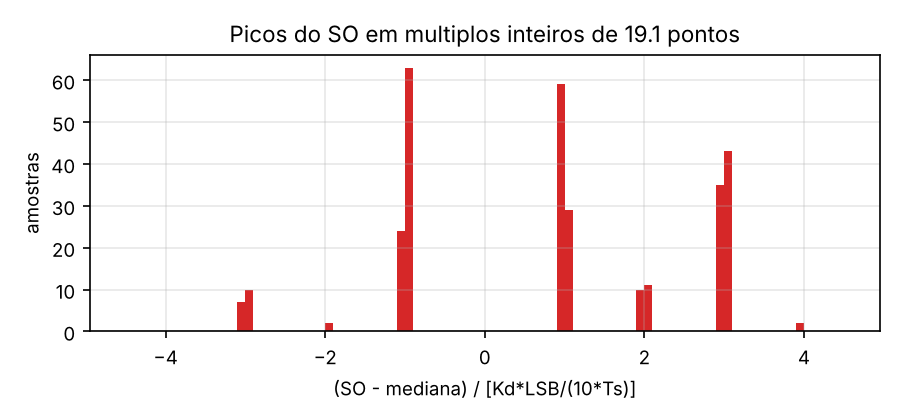
\includegraphics[width=.6\textwidth]{figs_exp/plc_histograma.png}\caption{Histograma dos picos do SO em unidades de $u_0=19{,}1$ pontos.}\end{figure}
\item \textbf{Por que há tantos picos se a VP muda devagar?} O ADC real tem ruído: quando a tensão está perto da fronteira entre dois códigos, a leitura \emph{alterna} entre eles de um scan para o outro (50 leituras por segundo). Cada alternância é um degrau de 1 LSB e gera outro pulso. No simulador fiel, um ruído de apenas $\sigma=0{,}15$ LSB ($0{,}7$ mV) reproduz a fração de picos observada:
\begin{center}\small\begin{tabular}{lccccc}\toprule $\sigma$ (LSB) & 0 & 0,10 & 0,15 & 0,20 & 0,30\\\midrule frac.\ picos (exp.: 0,20) & 0,01 & 0,18 & 0,25 & 0,39 & 0,55\\ desvio-padrão do SO (exp.: 17,3) & 2,7 & 15,0 & 16,9 & 21,6 & 26,1\\ $t_{63}$ [s] (exp.: 79) & 70 & 74 & 77 & 80 & 92\\\bottomrule\end{tabular}\end{center}
\end{enumerate}
\subsection{Terceiro: por que o SO fica entre 10 e 99,9}
Os pulsos (de até $\pm76$ pontos) somam-se ao SC e são cortados pelo \texttt{LIMIT(10,\,u,\,100)} do programa. Daí o gráfico entre 10 e 99,94\,\%. O limite inferior em 10\,\% (e não 0\,\%) é uma decisão do programa.
\subsection{Por que a planta ``não liga'' para os picos --- e por que ainda assim eles importam}
O circuito RC é um passa-baixa de 3ª ordem ($\tau\ge10$ s): pulsos de 60 ms mudam a VP em milésimos de ponto. Mas:
\begin{enumerate}
\item \textbf{Retificação pelos limites:} cortar os pulsos nos limites \emph{desloca a média} do SC. Na Q13b o SO médio no patamar saturado foi $96{,}6\,\%$ (não $99{,}94$), o que reduz a VP máxima em $\approx1{,}3$ ponto: $38{,}16$ medido contra $39{,}39$ sem ruído (Q13a). A simulação fiel prevê $38{,}35$.
\item \textbf{Congelamento da integral:} cada pulso que satura $u$ congela a integral (\texttt{STOP\_INTGR}) naquele scan: a resposta fica $\approx10\,\%$ mais lenta (t$_{63}$ 77 contra 70 s).
\item \textbf{Atuador} chaveando entre os limites; e \textbf{SC experimental não comparável} com o simulado (usa-se a mediana móvel).
\end{enumerate}
\subsection{É necessário trocar para um PI?}
\textbf{Resposta direta: não é necessário para a \emph{estabilidade}, mas é a correção mais simples; a simulação mostra que a resposta quase não muda.} Há três correções, em ordem crescente de esforço (resultados da simulação fiel ao PLC, $\sigma=0{,}15$ LSB, degrau 19,5$\to$30\,\%):
\begin{center}\small\resizebox{\textwidth}{!}{\begin{tabular}{lcccc}\toprule Programa & SO médio & desvio-padrão do SO & frac.\ picos & $t_{63}$\\\midrule
Original (\texttt{kd = 39.16}, sem filtro) & 76,1 & 16,9 & 0,25 & 77 s\\
\textbf{(1) PI de Dahlin:} \texttt{kp = 3.021}, \texttt{ki = 0.03872}, \texttt{kd = 0} & 76,1 & \textbf{0,1} & 0,00 & 71 s\\
\textbf{(2) PID com passa-baixa na VP} ($\tau_f=1{,}11$ s, só para a derivada) & 76,1 & \textbf{0,3} & 0,00 & 70 s\\
(3) só inicializar a derivada ao fechar a malha & 75,0 & 18,8 & 0,29 & 77 s\\\bottomrule\end{tabular}}\end{center}
\begin{figure}[H]\centering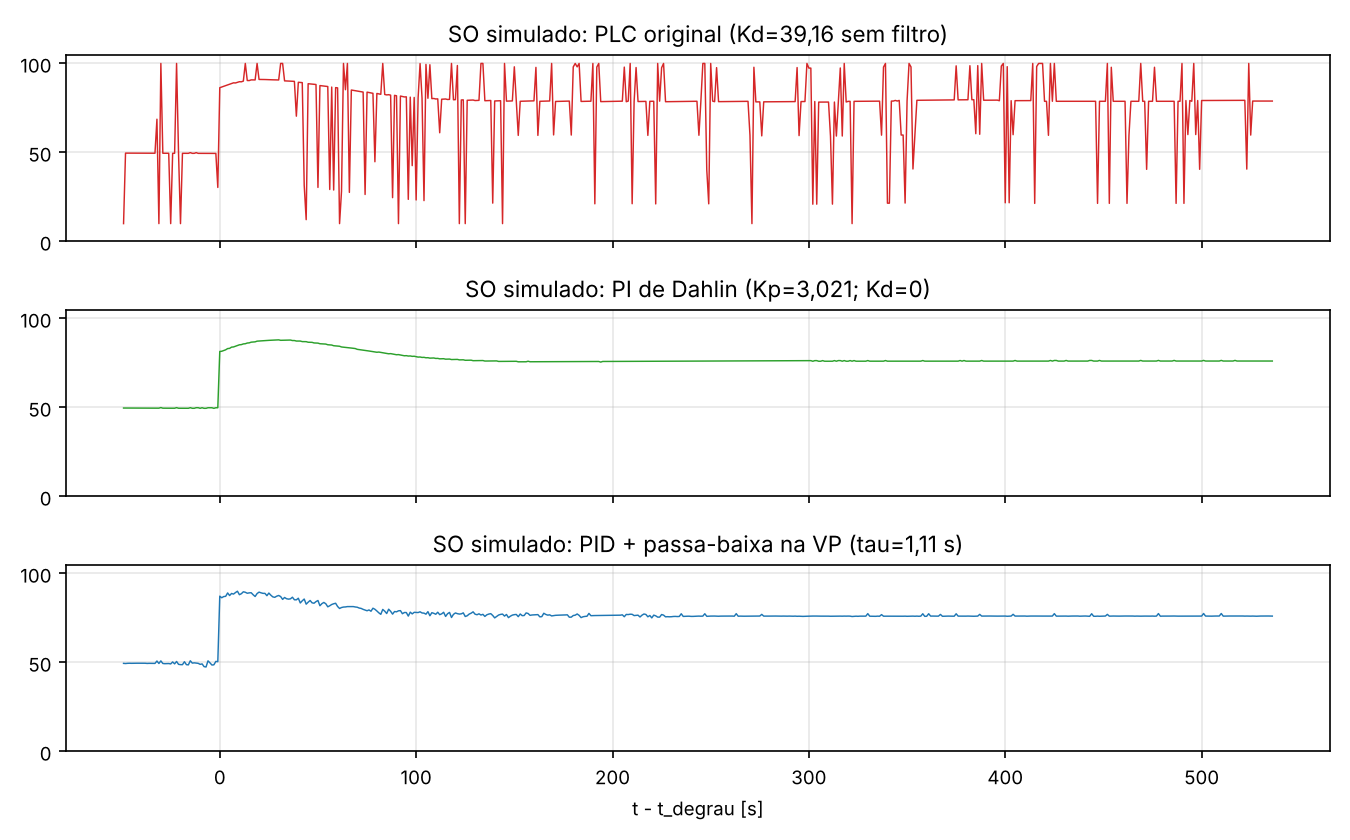
\includegraphics[width=.9\textwidth]{figs_exp/plc_correcoes.png}\caption{SO simulado (simulação fiel ao PLC): programa original, PI de Dahlin e PID com passa-baixa na VP.}\end{figure}
\textbf{(1) PI de Dahlin.} Vem da mesma dedução da Tabela 7-4.1 (Padé de ordem zero, $e^{-t_0s}\approx1-t_0s$): $C=\dfrac{\tau s+1}{Ks(\tau_c+t_0)}\Rightarrow K_c=\dfrac{\tau}{K(\tau_c+t_0)}=\dfrac{78{,}03}{0{,}3918\cdot65{,}92}=3{,}02$, $\tau_I=\tau=78{,}03$ s, \textbf{logo $k_i=K_c/\tau_I=3{,}02/78{,}03=0{,}03872$, o mesmo $k_i$ do PID}. No programa basta alterar \texttt{kp := 3.021} e \texttt{kd := 0.0}. Na FT completa, o PI dá $PM=70^\circ$ e $GM=9{,}5$ (contra $81^\circ$ e $59{,}7$ do PID), com resposta equivalente, e o efeito de 1 LSB da VP no SC cai de 76 pontos (pico da derivada de 4 pontos) para $K_c\cdot0{,}0976=0{,}3$ ponto.\\
\textbf{(2) Passa-baixa na VP antes da derivada} (mantém o PID do enunciado). Acrescentar no programa:
\begin{lstlisting}
(* variaveis novas:  VP_F : REAL := 0.0;   kf_VP : REAL := 0.017699;   (= 0.02/(1.11+0.02)) *)
IF NOT MF THEN VP_F := VP_PERC; END_IF;                       (* em manual, acompanha a VP *)
VP_F := VP_F + kf_VP * (VP_PERC - VP_F);                      (* passa-baixa de 1a ordem, Ts = 20 ms *)
Kd_VP_PERC := -1.0 * kd * VP_F * M_ACAO;                      (* no lugar de SEL(MF, 0.0, -VP*kd*M_ACAO) *)
\end{lstlisting}
O filtro é o $\mu T_d=0{,}1\cdot11{,}11=1{,}11$ s do projeto, e a linha sem \texttt{SEL(MF,\ldots)} mantém a derivada ``armada'' em manual, eliminando o pulso ao fechar a malha. \textbf{Estas duas correções foram validadas só em simulação, não na bancada.}\\
\textbf{(3)} Inicializar a derivada \emph{sozinha} não resolve o ruído (linha 3 da tabela): o problema é a falta de filtro.
\textbf{Recomendação:} (a) manter o relatório do item 1.1 como PID (é o que o enunciado pede) e documentar o ruído com esta análise; (b) \textbf{registrar um ensaio com PI} (correção 1) ou com a correção 2 e confrontar VP e SC: o SC deve ficar limpo (desvio-padrão do SO em torno de 0,1--0,3 ponto, como na simulação) e $t_{63}\approx70$ s.

%------------------------------------------------------------------
\section{Simulação fiel ao PLC (com ruído do ADC) $\times$ experimentos}\label{simplc}
Na Parte A, a simulação \emph{ideal} reproduz a VP dos ensaios com RMS de 0,24 a 0,43\,\% (exceto onde o ruído importa, Q13b), mas não reproduz três coisas: (i) o SO ruidoso, (ii) o fato de a resposta experimental ser $\approx10\,\%$ mais lenta e (iii) o deslocamento da média do SC (retificação). Para checar a explicação da Seção~\ref{expruido}, montei o \textbf{simulador fiel ao programa do PLC} (\texttt{plc\_sim.py}): a cada 20 ms ele executa o programa --- ADC de 10 bits com ruído, zona morta de $0{,}09$, integral com \texttt{STOP\_INTGR}, derivada de 4 pontos \emph{sem filtro}, bias \texttt{SO\_AUX}, \texttt{LIMIT(10,\,u,\,100)} e o 2GL por \texttt{FF2GL} --- sobre a mesma planta de 3ª ordem. O único parâmetro livre é o \textbf{ruído do ADC}, $\sigma\approx0{,}15$ LSB ($0{,}7$ mV), ajustado uma vez na Q11 e mantido nas demais.
\subsection{Q11}
\begin{figure}[H]\centering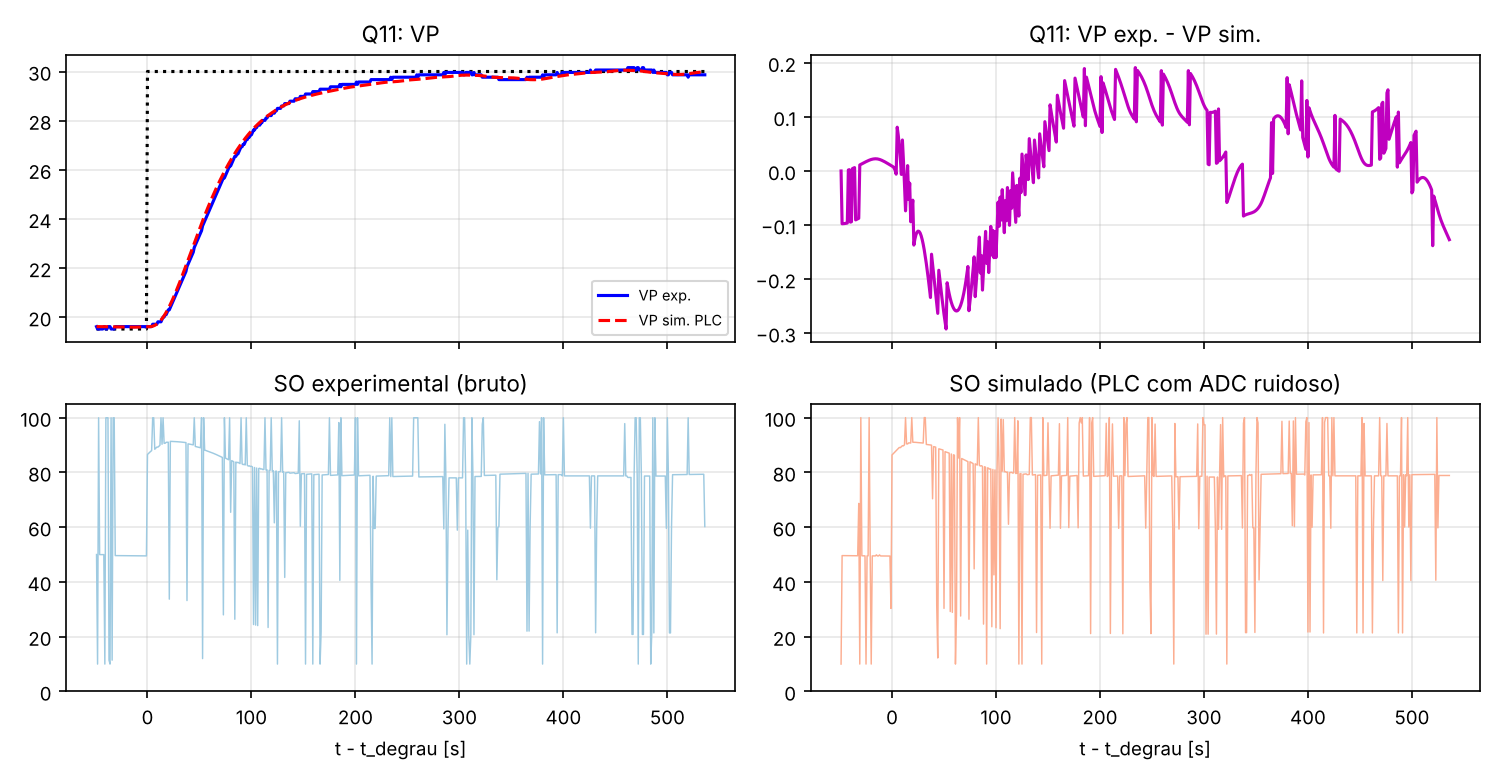
\includegraphics[width=.98\textwidth]{figs_exp/plc_q11.png}\caption{Q11 com a simulação fiel ao PLC. Acima: VP experimental, simulada e a diferença. Abaixo: SO experimental e SO simulado.}\end{figure}
\begin{center}\small
\begin{tabular}{lccc}\toprule & Experimento & Sim.\ ideal (Parte A) & Sim.\ fiel ao PLC\\\midrule
$t_{28,3}$ / $t_{50}$ / $t_{63,2}$ [s] & 43 / 64 / 79 & 39 / 57 / 70 & 41 / 62 / 77\\
$t_{90}$ / $t_{95}$ / $t_{98}$ [s] & 147 / 202 / 260 & 118 / 142 / 174 & 152 / 214 / 290\\
Erro VP: RMS / máx.\ [\%] & --- & 0,38 / 0,91 & \textbf{0,11 / 0,29}\\
SO médio em regime (últimos 300 s) & 75,4 & 76,2 & 76,1\\
Desvio-padrão do SO bruto & 17,3 & (sem ruído) & 16,9\\
Fração de amostras com pico ($|SO-\text{mediana}|>8$) & 0,20 & 0 & 0,25\\\bottomrule\end{tabular}\end{center}
A simulação fiel reduz o erro de VP em três vezes e reproduz o SO bruto em estatística (média, dispersão, fração de picos). A lentidão extra tem causa: cada pico que satura $u$ congela a integral naquele scan (\texttt{STOP\_INTGR}); sem ruído (PI ou derivada filtrada), a simulação fiel prevê $t_{63}=70$--71 s, igual à simulação ideal.
\subsection{Q12}
A simulação fiel dá, nos três primeiros scans após fechar a malha, \texttt{10, 10, 10} (derivada zerada em manual) e depois $49{,}2$; a mediana do SO de 595 a 615 s é $51{,}9$ (experimento: $50{,}2$; ideal: $49{,}2$) e a VP tem RMS de $0{,}22\,\%$ (ideal: $0{,}24\,\%$).
\subsection{Q13a e Q13b}
\begin{figure}[H]\centering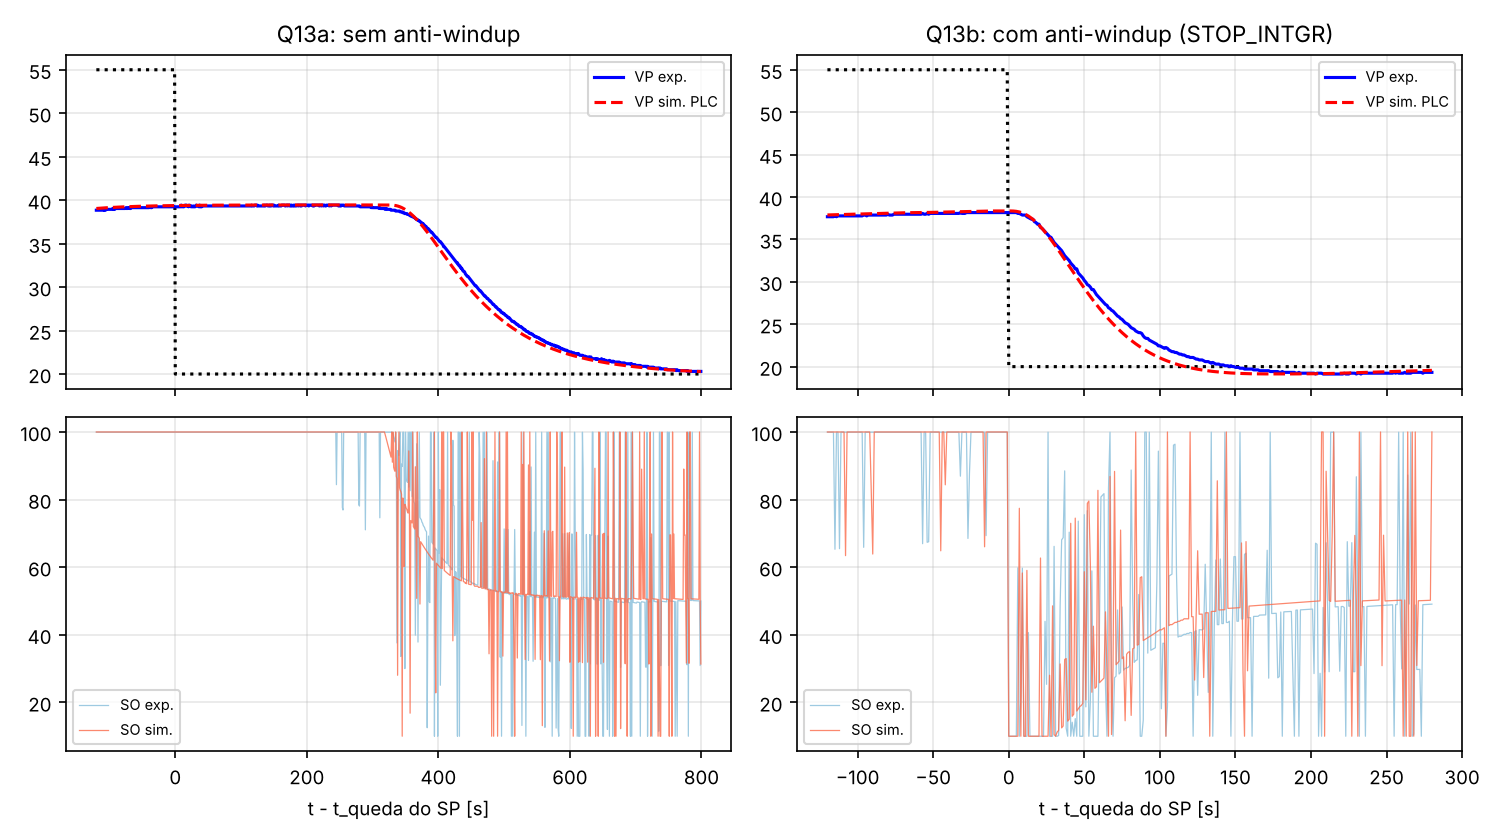
\includegraphics[width=.98\textwidth]{figs_exp/plc_q13.png}\caption{Q13 alinhado na queda do SP ($t=0$), com a simulação fiel ao PLC. Esquerda: sem anti-windup. Direita: com anti-windup (\texttt{STOP\_INTGR}). Acima: VP. Abaixo: SO experimental e simulado.}\end{figure}
\begin{center}\small
\resizebox{\textwidth}{!}{\begin{tabular}{lcccccc}\toprule & \multicolumn{3}{c}{Q13a: sem AW} & \multicolumn{3}{c}{Q13b: com AW}\\
 & Exp. & Ideal & Fiel & Exp. & Ideal & Fiel\\\midrule
O SO sai da saturação [s] & 337 & 326 & 325 & 0 & 0 & 0\\
VP em $20\pm1$ [s] & 700 & --- & 681 & 123 & --- & 101\\
SO médio no patamar saturado [\%] & 99,9 & 100,0 & 100,0 & 96,6 & 99,9 ($96{,}5^*$) & 96,5\\
VP máxima [\%] & 39,33 & 39,36 & 39,38 & 38,16 & 39,40 ($38{,}03^*$) & 38,35\\
Erro RMS da VP [\%] & --- & 0,43 & 0,44 & --- & 9,2 ($1{,}62^*$) & 0,63\\\bottomrule\end{tabular}}\end{center}
{\small $^*$ Na simulação ideal da Q13b, o limite superior do SC foi ajustado à mão a $96{,}5\,\%$ (a média medida) para emular a retificação do ruído; sem esse ajuste o RMS é 9,2\,\%. Na simulação fiel, a retificação surge sozinha do ruído do ADC.}
\par A simulação fiel reproduz os dois ensaios com a estrutura correta (sem \texttt{STOP\_INTGR} na Q13a e com na Q13b) e \emph{explica} a média de 96,6\,\% do SO e a VP máxima de 38,16 sem ajuste manual.
\subsection{O que a simulação fiel mostra}
\begin{itemize}
\item A explicação do ruído (derivada de 4 pontos sem filtro sobre o ADC) é \emph{suficiente} para reproduzir os três efeitos que a simulação ideal não captura.
\item A simulação ideal continua sendo a referência de projeto (Seções~\ref{it31}, \ref{it41} e Parte C): é nela que as sintonias são verificadas. A simulação fiel serve para \emph{prever o desvio} que o programa original causa na bancada.
\end{itemize}

\section{Comentário sobre a correção do bloco PID do OpenPLC}\label{progcorr}
\textbf{Comentário.} O bloco PID do programa (\texttt{Prova2.st}) calcula a derivada com uma diferença finita de 4 pontos a cada 20 ms \emph{sem nenhum filtro}, e ainda a zera em manual. Isso é inadequado para uma VP lida por um ADC de 10 bits: cada degrau (ou alternância) de 1 LSB vira um pulso de até $0{,}4\,k_d\,\mathrm{LSB}/T_s$ pontos no SC. A correção proposta é a que a teoria do PID prática já prevê: um \textbf{filtro derivativo} ($N$ ou $\mu$ na forma $\frac{K_ds}{\mu T_ds+1}$ das seções 7 a 13), aqui implementado como passa-baixa de 1ª ordem sobre a VP antes do bloco \texttt{DERIVATIVE}, com a mesma constante $\mu T_d=1{,}11$ s usada em todos os projetos deste relatório; e deixar a derivada ``armada'' em manual para eliminar o pulso ao fechar a malha. \textbf{O que está feito:} o texto \texttt{Prova2\_corrigido.st} e o projeto OpenPLC corrigido, com a previsão por simulação. \textbf{O que falta (a cargo do aluno):} repetir os ensaios com o programa corrigido e comparar com o programa original (Seção~\ref{simplc}) --- as caixas amarelas abaixo.
\subsection{O que mudou e o que se espera}
Gerei o arquivo \texttt{Prova2\_corrigido.st}, que é o \texttt{Prova2.st} com \textbf{duas alterações} (diferença completa em \texttt{Prova2\_diff.txt}, Apêndice~\ref{apcodigos}):
\begin{enumerate}
\item \textbf{Passa-baixa na VP antes da derivada:} \texttt{VP\_F := VP\_F + kf\_VP*(VP\_PERC - VP\_F)}, com \texttt{kf\_VP = 0.017699} $=T_s/(\tau_f+T_s)=0{,}02/(1{,}11+0{,}02)$, isto é, $\tau_f=1{,}11$ s ($=\mu T_d$ do projeto). A derivada passa a atuar sobre \texttt{VP\_F}. Em manual, \texttt{VP\_F} acompanha a VP.
\item \textbf{Derivada sem o \texttt{SEL(MF, 0.0, ...)}:} fica ``armada'' também em manual, o que elimina o pulso de 3 scans ao fechar a malha.
\end{enumerate}
Todo o resto (\texttt{kp}, \texttt{ki}, \texttt{kd}, \texttt{alfa}, \texttt{STOP\_INTGR}, \texttt{LIMIT}, VP-tracking) permanece igual. \textbf{Previsão da simulação fiel ao PLC} ($\sigma=0{,}15$ LSB; desvio-padrão do SO em $t>300$ s após o degrau) para os itens que ainda serão ensaiados:
\begin{center}\small\resizebox{\textwidth}{!}{\begin{tabular}{l|ccc|ccc|c}\toprule & \multicolumn{3}{c|}{Programa original} & \multicolumn{3}{c|}{Programa corrigido} & Projeto\\
Cenário & SO sd & sobress. & $t_{63}$ & SO sd & sobress. & $t_{63}$ & (sem ruído)\\\midrule
1.1 Dahlin, 20$\to$30\,\% & 19,9 & 0,5\,\% & 77 s & \textbf{0,2} & 0,0\,\% & 70 s & 70 s\\
2.1 2GL (\texttt{alfa=0.36}), 20$\to$30\,\% & 18,9 & 0,5\,\% & \textbf{132 s} & \textbf{0,9} & 0,0\,\% & 103 s & 104 s\\
3.1 IAE, 20$\to$25\,\% & 21,2 & 1,1\,\% & 50 s & \textbf{0,7} & 2,7\,\% & 45 s & 44 s; 2,6\,\%\\
4.1 Z--N, 10$\to$12\,\% & 28,6 & \textbf{82\,\%} & 23 s & \textbf{1,3} & 64\,\% & 21 s & 21 s; 62\,\%\\
4.2 I\_PD (\texttt{alfa=0}), 10$\to$12\,\% & 23,4 & \textbf{15,8\,\%} & 54 s & \textbf{2,6} & 0,0\,\% & 46 s & 46 s; 1,6\,\%\\\bottomrule\end{tabular}}\end{center}
\begin{res}\textbf{O programa original distorce também os ensaios que ainda faltam}: o Z--N daria 82\,\% de sobressinal em vez de 62\,\%; o I\_PD, 16\,\% em vez de $\approx2\,\%$; o 2GL ficaria em 132 s em vez de 104 s (a integral congelada pelos picos \emph{atrasa} a resposta); no Z--N e no I\_PD, com $k_d=197$, cada LSB vira pulsos de 4 vezes o tamanho (até 385 pontos). Com o programa corrigido, a simulação volta aos valores de projeto e o SO fica limpo (desvio-padrão de 0,2 a 2,6 pontos). \textbf{Recomendo usar o \texttt{Prova2\_corrigido.st} em todos os ensaios dos itens 2.1 a 4.2.}\end{res}
\subsection{O projeto OpenPLC completo (\texttt{PI\_DtwoGL\_prll\_uno\_beta}) e o projeto corrigido}\label{projplc}
Depois de analisar o \texttt{Prova2.st}, recebi a pasta completa do projeto (\texttt{plc.xml} em diagrama de blocos, mais os arquivos de compilação). Confirmei que o \texttt{Prova2.st} é exatamente o texto gerado desse diagrama e ganhei informações dos comentários e das declarações do próprio projeto:
\begin{itemize}
\item \textbf{Mapa de pinos (Arduino Uno):} \texttt{VP} = \texttt{\%IW0} = entrada analógica A0; \texttt{SO} = \texttt{\%QW1} = saída PWM do pino 10; \texttt{MF} = \texttt{\%QX0.0} = saída digital do pino 7 (``malha fechada $=1$''); \texttt{SP} = \texttt{\%QW0} (registrador alterado pelo ScadaBR). Valor inicial do \texttt{SO} $=6800$ ($\approx10{,}4\,\%$).
\item \textbf{Comentário do autor, no próprio diagrama:} ``\texttt{FILTRO DE MEDIA NA MEDIDA DE VP (???)}'', ao lado das conversões de escala: o autor já suspeitava que faltava um filtro na medida da VP, exatamente a correção proposta.
\item \textbf{Comentário sobre os ciclos:} ``\texttt{1/N, onde TIME CYCLE = N$\cdot$[TASK0 = 20 ms]; ex.: CYCLE = 100 ms então N = 5}''. Com \texttt{CYCLE = 500 ms}, $N=25$: o integrador é multiplicado por $1/N=0{,}04$ e a derivada por $N=25$, como analisei na Seção~\ref{secst}.
\item \textbf{Comentário do limite de 10\,\%:} ``\texttt{DEPENDE DO COOLER O MIN}'': o mínimo de 10\,\% do SC vem do atuador original (um \emph{cooler}/ventoinha que não gira abaixo desse valor).
\item \textbf{Comentário do 2GL:} ``\texttt{alfa = 0: I\_PD; alfa = 1: PI\_D}'', coerente com o código (peso $b=\mathtt{alfa}$). A legenda ``\texttt{FF2GL = kp*alfa*var\_SP}'' não bate com o bloco, que usa $(1-\mathtt{alfa})$; o comportamento correto é o do bloco.
\item A saída \texttt{SO} é PWM (no Uno, \texttt{analogWrite} de 8 bits, o que \emph{provavelmente} limita a resolução do SC a $100/255\approx0{,}4\,\%$; confirme).
\end{itemize}
\textbf{Projeto corrigido.} Em vez de apenas o texto \texttt{.st}, gerei o \textbf{projeto OpenPLC corrigido} (pasta \texttt{plc\_corrigido/PI\_DtwoGL\_prll\_uno\_beta\_corrigido/}, também em \texttt{.zip}), editando o diagrama do \texttt{plc.xml}: (i) uma rede nova de 5 blocos (\texttt{SUB}, \texttt{MUL}, \texttt{ADD}, \texttt{SEL}) calcula \texttt{VP\_F}, com comentário no diagrama (parte inferior); (ii) a entrada da derivada passa de \texttt{VP\_PERC} para \texttt{VP\_F}; (iii) o \texttt{SEL(MF, 0.0, \ldots)} da derivada foi removido. Duas variáveis novas foram declaradas (\texttt{VP\_F}, \texttt{kf\_VP}). Os arquivos de compilação antigos (\texttt{build/}) foram omitidos: o editor os regenera.
\textbf{Conferência feita:} (a) o XML novo é bem formado, os \texttt{localId} são únicos e todas as 166 referências de conexão existem; (b) escrevi um tradutor do diagrama para texto (\texttt{fbd\_para\_st.py}): aplicado ao \textbf{original}, ele reproduz as expressões do \texttt{Prova2.st} (ex.: \texttt{ERRO\_PERC}, \texttt{STOP\_INTGR}, \texttt{FF2GL}), o que valida o tradutor; aplicado ao \textbf{corrigido}, as \emph{únicas} saídas diferentes são \texttt{Kd\_VP\_PERC := MUL(-1.0, VP\_F, kd, M\_ACAO)} e \texttt{VP\_F := SEL(MF, VP\_PERC, ADD(VP\_F, MUL(SUB(VP\_PERC, VP\_F), kf\_VP)))}. \textbf{O que não foi possível:} abrir o projeto no OpenPLC Editor nem compilar com o \texttt{matiec} (não disponíveis aqui). Ao abrir, as linhas de conexão da rede nova podem precisar de ajuste visual; a lógica está conferida. \emph{Se o editor recusar o arquivo, use o \texttt{Prova2\_corrigido.st} como referência e refaça as 5 conexões à mão (são 8 linhas).}

\begin{todo}Abrir o projeto corrigido no OpenPLC Editor (pasta \texttt{PI\_DtwoGL\_prll\_uno\_beta\_corrigido}), \emph{Build} (confirmar que não há erro), carregar no Arduino; repetir o item 1.1 (Dahlin, 20$\to$30\,\%) e conferir: SO sem picos (desvio-padrão $\lesssim1$ ponto), SO $\approx76\,\%$ em regime, sem pulso de 10\,\% ao fechar a malha, $t_{63}\approx70$ s. Resultado: \underline{\hspace{6cm}}\end{todo}

%------------------------------------------------------------------
\section{Conclusões dos experimentos da Questão 1}\label{conclq1}
\begin{enumerate}
\item \textbf{Modelo validado no dia do ensaio:} inclinação $0{,}3963$ (teórico $0{,}3971$), offset de $-0{,}26$ ponto, dinâmica reproduzida com RMS de 0,2--0,8\,\% com o SO medido como entrada.
\item \textbf{Item 1.1 (simulação ideal):} a sintonia de Dahlin ($\tau_c=40$ s) funcionou: sem sobressinal significativo e sem erro em regime; salto de SC igual a $K_p\Delta SP$; RMS da VP de 0,38\,\%. A resposta experimental é $\approx13\,\%$ mais lenta que a ideal ($t_{63}$ de 79 contra 70 s).
\item \textbf{Item 1.2:} sem VP-tracking o SC saltou $+30$ pontos (previsto $K_p(SP-VP)=29{,}2$); com tracking (Q11), não há salto.
\item \textbf{Item 1.3:} sem anti-windup a VP fica presa em 39,3\,\% por $\approx340$ s depois da queda do SP e só chega a $20\pm1\,\%$ em 700 s; com anti-windup, em 123 s. A conta analítica dá 328 s para a saída da saturação (medido 337).
\item \textbf{SO ``instável'':} é \textbf{ruído no sinal de controle}, não instabilidade. O programa usa uma derivada de 4 pontos \emph{sem filtro} sobre a VP quantizada em 1 LSB; cada degrau (ou alternância) de 1 LSB gera pulsos de 57, 76 e 57 pontos durante 3 scans de 20 ms, cortados em 10 e 100\,\% pelo \texttt{LIMIT}. Prova: 100\,\% dos 295 picos medidos são múltiplos inteiros de $k_dLSB/(10T_s)=19{,}1$ pontos. A simulação fiel ao PLC reproduz o ruído, a lentidão e a retificação.
\item \textbf{Consequências do ruído:} retificação (SO médio de 96,6\,\% no patamar saturado), congelamento intermitente da integral (resposta $\approx10\,\%$ mais lenta) e SC experimental ruidoso.
\item \textbf{Correção do bloco PID:} passa-baixa de 1,11 s na VP antes da derivada e derivada armada em manual (\texttt{Prova2\_corrigido.st} e projeto corrigido); alternativa mínima: PI de Dahlin. \textbf{Previsão apenas por simulação; os ensaios com o programa corrigido serão feitos depois} (Seção~\ref{progcorr}).
\item \textbf{Tradução do 2GL:} no programa, $\mathtt{alfa}_{PLC}=1-\alpha_{TCC}$; o $\alpha_{TCC}=0{,}64$ do item 2.1 vira \texttt{alfa = 0.36}; o I\_PD do item 4.2 é \texttt{alfa = 0}.
\end{enumerate}
\textbf{Limitações:} (i) as versões do programa usadas em Q12 e Q13a são inferidas dos dados; (ii) o ruído do ADC é um único parâmetro ajustado ($\sigma\approx0{,}15$ LSB; faixa 0,1--0,2); (iii) a fórmula de 4 pontos do bloco \texttt{DERIVATIVE} é a da biblioteca padrão, confirmada indiretamente pelos dados e não pelo código-fonte do runtime; (iv) as correções (PI, passa-baixa e o projeto corrigido) só foram testadas em simulação e não foram compiladas no OpenPLC; (v) um ensaio de cada tipo, sem repetição.

